\section{Explicit Values}
\label{sec:values}

There are several methods available to generate or count all
triangulations of a finite set of points in~$\R^2$. An approach that
works for point sets in arbitrary dimensions is implemented in the
software package \topcom\ by Rambau~\cite{Rambau-TOPCOM} (see also
Pfeifle and Rambau~\cite{PfeifleRambau}). It enumerates all
triangulations in a purely combinatorial manner after the chirotope of
the point set (oriented matroid data) has been computed.

The \emph{reverse search algorithm} proposed by Avis and
Fukuda~\cite{AvisFukuda} is a rather general enumeration scheme that
can be specialized to triangulations of point configurations in $\R^2$
(see also Bespamyatnikh~\cite{Bespamyatnikh}). Since it was used to
obtain some of the results reported in Section~\ref{sec:trias}, and
because it is based upon some structural properties that are relevant
for our treatment later, we briefly describe the method here.

Let~$\mathcal{T}$ be a \emph{fine triangulation} of a point set
$S\subset\R^2$; i.e., $\mathcal{T}$ is a set of triangles, for which
the set of vertices equals~$S$, such that the union of all triangles
is the convex hull of~$S$, and any two triangles intersect in a common
(possibly empty) face. The unimodular triangulations of $P_{m,n}$ are
precisely its fine triangulations. An edge of some triangle
in~$\mathcal{T}$ is \emph{flippable} if it is contained in two
triangles of~$\mathcal{T}$ whose union is a strictly convex
quadrangle.  Replacing these two triangles by the two triangles into
which the other diagonal cuts that quadrangle (\emph{flipping} the
edge) yields another fine triangulation of~$S$.  The graph on the fine
triangulations of~$S$ defined via flipping is the 
\emph{flip graph} of~$S$.

Let us fix an arbitrary ordering of the points in~$S$, inducing via
lexicographical ordering a total order on the set of pairs of points,
and thus, again via lexicographical ordering, a total order on the
fine triangulations of~$S$, which are identified with their sets of
edges here.   There is a distinguished fine
triangulation~$\mathcal{T}_0$ of~$S$ with respect to that ordering,
namely the smallest \emph{Delaunay triangulation} (i.e., 
a triangulation characterized by the condition that for every triangle
the circumcircle contains no point from~$S$ in its interior).

Furthermore, for each fine triangulation
$\mathcal{T}\not=\mathcal{T}_0$, there is a distinguished flippable
edge
%$\text{flip}(\mathcal{T})$ 
(computable in $\order{|S|}$ steps) such that, starting from any fine
triangulation of~$S$, iterated flipping of the respective
distinguished edges eventually yields $\mathcal{T}_0$.  This
algorithmically defines a spanning tree in the flip graph of~$S$,
rooted at~$\mathcal{T}_0$; in particular, the flip graph of a two
dimensional finite point set is connected.

The basic idea of the reverse search method is to traverse that
spanning tree from its root~$\mathcal{T}_0$. At each iteration one
chooses a leaf~$\mathcal{T}$ of the current partial tree, and
determines those among the triangulations adjacent to~$\mathcal{T}$ on
whose path to~$\mathcal{T}_0$ in the spanning tree~$\mathcal{T}$ lies.
Properly implemented, the reverse search algorithm generates all fine
triangulations in $\order{|S|\cdot f(S)}$ steps, where~$f(S)$ is the
number of fine triangulations of~$S$; see~\cite{AvisFukuda}.

Via the ``secondary polytope'' of a finite point set
$S\subset\R^2$~\cite{GKZ}  
one can design a variant of the reverse
search algorithm that generates \emph{all} \emph{regular}
triangulations of~$S$ in $\order{|S|\cdot F^{\text{reg}}(S)}$ steps,
where $F^{\text{reg}}(S)$ is the number of such triangulations. It is,
unclear, however, if one can also generate all \emph{regular}
\emph{fine} triangulations of~$S$ in a number of steps that is bounded
by a polynomial in the number of such triangulations.
 
If one is interested in the number of triangulations of a
two-dimensional set of points rather than in the explicit generation
of all of them, then the \emph{path of a triangulation method} due to
Aichholzer~\cite{Aichholzer-path} is more efficient than the reverse
search algorithm.

For counting the unimodular (fine) triangulations of the very special
point sets $P_{m,n}$, however, different methods are much more
efficient. These are described in the following sections.


\subsection{Narrow Strips}
\label{subsec:narrow}

\paragraph{Strips of width \boldmath$m=1$. }

For any lattice trapezoid of width~$1$, whose parallel vertical sides
have lengths $a$ and~$b$, the number of unimodular
triangulations is $g_1(a,b)=\binom{a+b}a= \binom{a+b}b$; indeed, a
bijection between these triangulations and the $a$-subsets of
$\{1,\dots,a+b\}$ is established by top-down numbering the triangles
of a triangulation~$\mathcal{T}$ by $1,\dots,a+b$, and
mapping~$\mathcal{T}$ to the $a$-set of all numbers of triangles whose
vertical edges are on the left. In particular, we have
\begin{equation}
  \label{eq:1n}
  f(1,n)\ =\ \binom{2n}{n}.  
\end{equation}

\paragraph{Strips of width \boldmath$m=2$. }

For $f(2,n)$ we have no explicit formula, and we cannot evaluate the
asymptotics precisely, but we have a ``quadratic'' recursion that can
be evaluated efficiently: For this we enumerate the triangulations
according to the highest ``width~$2$ diagonal,'' which (if it exists)
decomposes the rectangle into two width~$1$ strips, a single triangle,
and a trapezoid of width~$2$ (see the left-hand figure below).  Let
$g_2(A,B)$ denote the number of triangulations of a trapezoid of
width~$2$ with vertical edges of lengths~$A$ and~$B$ 
and horizontal base line, as in the right-hand figure below --- where
$A+B\equiv1\bmod2$ implies that the midpoint of the diagonal is not a
lattice point, and where we may assume $A<B$ by symmetry:
\[
\input{v_strip2recursion1+2.pstex_t}
\]
Thus we get 
\[
f(2,n)\ =\ \binom{2n}{n}^2\ +\ 2
\hspace{-3mm} \sum_{0\le A<B\le n\atop A+B\equiv1\bmod2}\hspace{-4mm}
g_2(A,B)
\binom{2n-\tfrac{3A+B+1}2}{n-A}
\binom{2n-\tfrac{A+3B+1}2}{n-B}.
\]
The binomial coefficients in this recursion
correspond to triangulations of width~$1$ strips. So they
could be rewritten in terms of $g_1$, as 
$g_1(n-A,n-\tfrac{A+B+1}2)$ resp.\ $g_1(n-B,n-\tfrac{A+B+1}2)$.
A similar remark applies to the binomial coefficients that
appear in the following.

For $g_2(A,B)=g_2(B,A)$ we also get a recursion by considering the
highest diagonal of width~$2$:
\begin{eqnarray*}
g_2(A,B) & = &\ 
\binom{\frac{3A+B-1}2}{A}
\binom{\frac{A+3B-1}2}{B}\\
&&+ 
\sum\limits_{0\le a\le A,\ 0\le b\le B \atop a+b\equiv1\bmod2,\ a+b<A+B}
g_2(a,b)\,
\binom{\frac{3A+B-3a-b}{2}-1}{A-a}
\binom{\frac{A+3B-a-3b}{2}-1}{B-b}.
\end{eqnarray*}
\begin{center}
\input{v_strip2recursion3+4.pstex_t}
\end{center}
Here the parameters $A,B,a,b$ may be interpreted as the $y$-coordinates
of certain lattice points. The shaded parts of the figure consist
of strips of width~$1$, whose triangulations are counted by
the binomial coefficients $g_1(\cdot,\cdot)$.


\paragraph{Strips of width \boldmath$m=3$. }

For $f(m,3)$ we have a recursion of order~$4$; it relies on the
observation that if we screen the middle strip from the 
top for diagonals of width at least~$2$, then the first diagonal
to find will be of width exactly~$2$, since any width~$3$ diagonal
is flippable, and contained in a parallelogram that is
bounded by two width~$2$ diagonals. 
The corresponding decomposition of our rectangle 
is indicated in the left figure below: 
\begin{center}
\centerline{\input{v_strip3recursion1+2.pstex_t}}
\end{center}
Therefore, we obtain
\[
f(3,n) \ =\ \binom{2n}{n}^3 + 2
\sum_{0\le A,B\le n\atop A+B\equiv1\bmod2}h(A,B,n,n)
\binom{2n-\frac{3A+B+1}{2}}{n-A}
\binom{2n-\frac{A+3B+1}{2}}{n-B},
\]
where $h(A,B,C,D)$ counts the number of triangulations
in a ``hook'' shape as given in the right drawing in the figure above,
which depends on four parameters $0\le A,B,C,D\le n$, 
with $A+B\equiv1\bmod2$ and $B\le C$.
For the number of triangulations of such a hook shape we get a recursion
\begin{eqnarray*}
\lefteqn{h(A,B,C,D) \ \ =\ \  
\binom{\frac{3A+B-1}2}{A} 
\binom{\frac{A+3B-1}2}{B}
\binom{C+D}{C}}\\
&&+\ 
\sum_{0\le a\le A,    \ 0\le b\le B\atop
     a+b\equiv1\bmod2,\ a+b<A+B}
h(a,b,C,D)
\binom{\frac{3A+B-3a-b}{2}-1}{A-a}
\binom{\frac{A+3B-a-3b}{2}-1}{B-b}\\
&&+\ 
\sum_{0\le a\le D,\ 0\le b\le \frac{A+B-1}{2}\atop
     a+b\equiv1\bmod2,\ \frac{a+b+1}{2}\le B}
h(a,b,\tfrac{A+B-1}{2},A)
\binom{D+C-\frac{3a+b+1}{2}}{D-a}
\binom{\tfrac{A+3B-a-3b}{2}-1}{B-\tfrac{a+b+1}{2}}
\\
&&+\ 
h(\tfrac{3B-A-1}{2},\tfrac{A+B-1}{2},\tfrac{A+B-1}{2},A)
\binom{C+D-\frac{5B-A-1}{2}}{C-B}\quad
\textrm{if }D\ge\tfrac{3B-A-1}{2}\ge0.
\end{eqnarray*}
The four terms in this recursion correspond to the 
four cases depicted in the figure below, 
where the fourth case --- of a long diagonal of width~$3$ ---
occurs only in the case where the second endpoint of the
diagonal, which may be computed to have $y$-coordinate
$\frac{3B-A-1}2$, comes to lie within the hook.
\medskip

\noindent%
\input{v_strip3recursion3.pstex_t}%

\subsection{Strips of (fixed) width \boldmath$m$. }

We now describe a recursive strategy for the enumeration of unimodular
triangulations of grids of arbitrary size.  The method is applicable
for triangulations of general finite point sets --- but it is
effective only in the special case where the points lie on a small
family of parallel (vertical, say) lines; in our case this is the
situation of small (fixed) $m$ and variable~$n$. The key observation is
that any triangulation may be dismantled by removing triangles from
the upper boundary, while maintaining a lattice triangulation of a
$y$-convex lattice polygon.  Since for fixed~$m$ the number of such
polygons in~$P_{m,n}$ is bounded by a polynomial in~$n$, this 
yields an efficient dynamical programming algorithm in this
case.

Let $\Delta_1,\Delta_2\subset\R^2$ be two triangles whose intersection
$\Delta_1\cap\Delta_2$ is a common (empty, zero-, or one-dimensional)
face of both~$\Delta_1$ and~$\Delta_2$.  
We say that \emph{$\Delta_2$ lies above $\Delta_1$} ($\Delta_1\prec
\Delta_2$) if there are two points $(x,y_1)\in
\Delta_1\setminus\Delta_2$ and $(x,y_2)\in \Delta_2\setminus\Delta_1$
on a vertical line with $y_1<y_2$.
For example, in our figure the shaded triangle lies above the 
other one; the other two pairs of triangles are incomparable.
\[  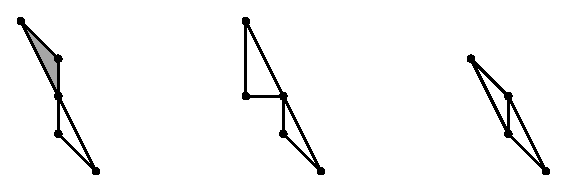
\includegraphics[height=3cm]{above2.eps}\]
Due to
the convexity of the triangles and the intersection condition imposed
on them, this is a well-defined asymmetric and irreflexive relation.

\begin{lemma}
  \label{lem:abov}
  There is no sequence $\Delta_0,\dots,\Delta_{t-1}\subset\R^2$ of
  triangles (such that the intersection of any two among them is a face
  of both) satisfying
  \begin{equation}
    \label{eq:abov}
    \Delta_0\abov\Delta_1\abov\dots\abov\Delta_{t-1}\abov\Delta_0\enspace.
  \end{equation}
\end{lemma}

\begin{proof}
  Suppose that $\Delta_0,\dots,\Delta_{t-1}\subset\R^2$ is a minimal cyclic
  sequence of triangles (such that the intersection of any two among
  them is a face of both), i.e., it satisfies~(\ref{eq:abov}) (it is
  \emph{cyclic}), but no subsequence of
  $\Delta_0,\dots,\Delta_{t-1}\subset\R^2$ is cyclic.  
  The orthogonal projections $x(\Delta_i)$ to the $x$-axis
  have the following three properties (where all
  indices are taken modulo~$t$): 
  \\(a)~$x(\Delta_i)\cap x(\Delta_{i+1})\not=\emptyset$, 
  \\(b)~$x(\Delta_i)\not\subseteq x(\Delta_{i-1}), x(\Delta_{i+1})$, and 
  \\(c)~$x(\Delta_{i-1})\cap x(\Delta_{i+1})=\emptyset$, 
  \\where (a) follows
  immediately from the definition of~$\abov$ and~(b) as well as~(c)
  are due to the minimality of the cycle.
  
  But (a), (b), and (c) together imply that the intervals
  $x(\Delta_0),\dots,x(\Delta_{t-1})$ ``either run left-to-right or
  right-to-left''; in particular, we have
  $x(\Delta_0)\cap x(\Delta_i)=\emptyset$ for $i\in\{2,\dots,t-1\}$,
  contradicting $\Delta_{t-1}\abov\Delta_0$.
\end{proof}


Of course, both in the definition of~$\abov$ as well as in 
Lemma~\ref{lem:abov} one can replace
``triangle'' by ``compact convex set.'' 

The relation~$\abov$ was defined with respect to parallel projection
here.  If one defines an ordering with respect to central rather than
to parallel projection, then the analog to Lemma~\ref{lem:abov} (for
arbitrary centers of projection) does not hold. For Delaunay
triangulations, however, there is an analog to Lemma~\ref{lem:abov}.
(See De Floriani et al.~\cite{DFNP91} for dimension~$2$, and
Edelsbrunner~\cite{Edelsbrunner92} for arbitrary dimensions.)

Due to Lemma~\ref{lem:abov}, the relation~$\abov$ induces 
a partial order on the set of triangles
in~$\R^2$, which we will also denote by~$\abov$.


A sequence $\mathcal{T}_1,\dots,\mathcal{T}_{2mn}$ of sets of
triangles will be called an \emph{admissible sequence} for $P_{m,n}$
if $\mathcal{T}_1$ is a unimodular triangulation of~$P_{m,n}$, and if,
for each $i=2,3,\dots,2nm$, we have
$\mathcal{T}_i=\mathcal{T}_{i-1}\setminus\{\Delta\}$ for some
$\abov$-maximal triangle~$\Delta$ in~$\mathcal{T}_{i-1}$.  A subset
$S\subset\R^2$ is called an \emph{admissible shape} (of $P_{m,n}$) if
it can be obtained as a union
$S=\bigcup_{\Delta\in\mathcal{T}_i}\Delta$ for an admissible sequence
$\mathcal{T}_1,\dots,\mathcal{T}_{2mn}$ and some
$i\in\{1,\dots,2mn\}$.  Every admissible shape is $y$-convex (i.e.,
its intersection with any vertical line is connected). It is
determined by its \emph{upper boundary segments}, i.e., the sequence
of line segments $[l^{(1)},r^{(1)}],\dots,[l^{(t)},r^{(t)}]$ with
$l^{(1)}_x=0$, $l^{(t)}_x=n$, and $r^{(j-1)}_x=l^{(j)}_x$ for
$j\in\{2,\dots,t\}$, such that, for each point~$p$ in the relative
interior of any of the segments, $p+(0,\varepsilon)\not\in S$ holds
for all $\varepsilon>0$.

Let~$S$ be an admissible shape. We denote by $\mathcal{T}_{\max}(S)$
the set of all $\abov$-maximal unimodular triangles in $S$,
that is, the finite set of all unimodular triangles that could
be $\abov$-maximal in \emph{some} unimodular triangulation of~$S$.
For example, the figure below indicates the 12
$\abov$-maximal triangles of the shaded admissible shape.
\[
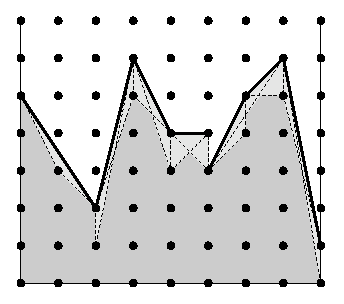
\includegraphics[height=5cm]{shape2.eps}
\]
Any admissible shape~$S'$ that arises
from~$S$ by removing some triangles contained in~$\mathcal{T}_{\max}(S)$ is
called an \emph{admissible subshape} of~$S$. These triangles have
disjoint interiors, and they are uniquely determined for each
admissible subshape~$S'$ of~$S$ (compare the proof of
Lemma~\ref{lem:maxtria}). Their number is denoted by $\#(S',S)$.

Since every unimodular triangulation of~$S$ contains at least one
triangle from~$\mathcal{T}_{\max}(S)$, we obtain the following
inclusion-exclusion formula for the numbers $f(S)$ of unimodular
triangulations of admissible shapes~$S$.

\begin{lemma}
  \label{lem:inex}
  Every admissible shape~$S$ has
  \begin{equation}
    \label{eq:admsh}
    f(S)=\sum_{S'}(-1)^{\#(S',S)-1}f(S')    
  \end{equation}
  unimodular triangulations, where the sum is taken over all
  admissible proper subshapes~$S'$ of~$S$.
\end{lemma}

Lemma~\ref{lem:inex} allows us to compute $f(m,n)=f([0,m]\times[0,n])$
via a dynamic programming approach: Determine the numbers $f(S)$
via~(\ref{eq:admsh}) in some order such that every admissible shape
appears after all its admissible subshapes. In order to analyze the
running time of such an algorithm, we first need to estimate the number
of admissible shapes.

\begin{lemma}
\label{lem:upbd}
  Let $[l^{(1)},r^{(1)}],\dots,[l^{(t)},r^{(t)}]$ be the sequence of upper boundary
  segments of an admissible shape~$S$. Then
  $$
  l^{(j)}_y\in\{r^{(j-1)}_y-1,r^{(j-1)}_y,r^{(j-1)}_y+1\}
  $$
  holds for each $2\leq j\leq t$.
\end{lemma}

\begin{proof}
  This follows by induction on the number of triangles removed in
  order to obtain~$S$: Every vertical edge of a triangle in a
  unimodular triangulation has length one, and thus removing a $\abov$-maximal
  triangle from an admissible shape never creates a vertical
  boundary part of height more than~$1$.
\end{proof}

Lemma~\ref{lem:upbd} implies the following bound on the number of
admissible shapes. 

\begin{lemma}
  \label{lem:numadm}
  There are at most $(3n+2)^{m-1}(n+1)^2$ admissible shapes of~$P_{m,n}$.
\end{lemma}

\begin{proof}
  The upper boundary of an admissible shape has $n+1$ possible start
  and $n+1$ possible end points. At every interior $x$-coordinate
  ($x\in\{1,\dots,m-1\}$) either a segment of the upper boundary ends
  and a new one starts ($3(n+1)-2$ possibilities, by
  Lemma~\ref{lem:upbd}) or a segment ``passes through'' (one possibility).
\end{proof}

The second important quantity for the analysis of the running time of
the dynamic programming algorithm proposed above is the maximal number
of summands that may occur in~(\ref{eq:admsh}).

\begin{lemma}
  \label{lem:maxtria}
  Every admissible shape~$S$ of $P_{m,n}$ has at most 
  $$
  \Big(\frac{3+\sqrt{13}}{2}\Big)^m<\ 3.31^m
  $$
  admissible subshapes.
\end{lemma}

\begin{proof}
  Let $(B_1,\dots,B_t)$ be the sequence (from left to right) of upper
  boundary segments of~$S$.  Each triangle in $\mathcal{T}_{\max}(S)$
  contains at least one of the edges $\{B_1,\dots,B_t\}$.
  
  Let $B\in\{B_1,\dots,B_t\}$ be a segment of the upper boundary
  of~$S$. There are at most two triangles in $\mathcal{T}_{\max}(S)$
  containing~$B$ and one of its adjacent segments.  Each other
  triangle in $\mathcal{T}_{\max}(S)$ that contains $B$ must have its
  third vertex~$v$ in $B+\R\cdot(0,-1)$ on the line that is parallel
  to~$B$ at distance $\ell_2(B)^{-1}$, where $\ell_2(B)$ denotes the
  Euclidean length of~$B$ (because the triangle has area $\frac12$).
  Since~$v$ must be integral and there is no integral point in the
  relative interior of~$B$, there are at most two possibilities
  for~$v$. Let us call one of them \emph{the first triangle
    below~$B$}, and the other one, \emph{the second triangle
    below~$B$} (if they exist).
  
  For every admissible subshape~$T$ of~$S$, define a word
  $w(T)\in\{0,\alpha,\beta,\gamma\}^{\star}$ by replacing $B_i$ by
  \begin{itemize}\itemsep=-2pt
  \item[`$\alpha$' ] if $S\setminus T$ contains the first triangle below~$B_i$,
  \item[`$\beta$' ] if $S\setminus T$ contains the second triangle below~$B_i$,
  \item[`$\gamma$' ] if $S\setminus T$ contains the triangle formed
    by~$B_i$ and~$B_{i-1}$, and
  \item[`$0$'      ] otherwise.
  \end{itemize}
  Clearly, every `$\gamma$' in $w(T)$ has a `$0$' as its left neighbor;
  furthermore, $w(\cdot)$ is an injective mapping. Therefore, the number
  of admissible subshapes of~$S$ is bounded from above by the
  function $\varphi(m)$ defined recursively via
  $$
  \varphi(0)=1\ ,\qquad
  \varphi(1)=3\ ,\qquad
  \varphi(m)=3\varphi(m-1)+\varphi(m-2)
  \quad(m\geq 2).
  $$
  Using standard techniques 
  (see, e.\,g., \cite[Thm. 4.1.1]{StanleyEnumComb}), one derives 
  from this recursion that
  $\varphi(m)<\big(\frac{3+\sqrt{13}}{2}\big)^m  $ for $m\ge1$. 
\end{proof}

Lemmas~\ref{lem:numadm} and~\ref{lem:maxtria} imply that (for
every~$m$) the dynamic programming algorithm needs at most
$$
3.31^m(3n+2)^{m-1}(n+1)^2\ <\ 10^m (n+1)^{m+1}
$$
arithmetic operations. The actual running time of an implementation
heavily depends on the data structures for storing the admissible
shapes and on the way by which one determines the admissible subshapes in
that data structure. Therefore, here we include only the following
rough statement.

\begin{theorem}
  For every fixed~$m$, the function $f(m,n)$ can be computed in time
  bounded by a polynomial in~$n$.
\end{theorem}

In our implementation, we organize the admissible shapes as the leaves
of a tree whose nodes are the prefixes of the sequences of upper
boundaries segments of admissible shapes. The data structure allows
quite efficient access to the admissible subshapes while not wasting
too much memory.  Nevertheless, the bottleneck in the computations
is always memory. It is crucial to use an ordering of the
admissible shapes in which for each shape~$S$ the shapes of which it
is an admissible subshape come as soon as possible after it; this
allows one to keep in memory only a subset of the admissible shapes at
each point of time.

Furthermore, in~(\ref{eq:admsh}) there is no need to sum over \emph{all}
admissible subshapes~$S'$. It suffices to consider those~$S'$ that
arise from removing triangles in~$\mathcal{T}_{\max}(S)$ that are
contained in $\{(x,y)\in\R^2:x\geq c\}$, where~$c$
is the maximal $x$-coordinate where $l^{(j)}_y=r^{(j-1)}_y+1$ for
some~$j$ and the upper boundary segments
$[l^{(1)},r^{(1)}],\dots,[l^{(t)},r^{(t)}]$ of~$S$ (if that maximum exists). 

Of course, when computing the number of unimodular triangulations of
$P_{m,n}$ by our method, we obtain as a byproduct the number of
unimodular triangulations of several interesting polygons inside
$P_{m,n}$, including $P_{m,1}$, \dots, $P_{m,n-1}$. 

The algorithm described above cannot only be used to calculate the
number of unimodular triangulations of any admissible shape~$S$
in~$P_{m,n}$; it can also be extended to produce a uniformly
distributed random triangulation within the same
asymptotic running time, and thus, in polynomial time (depending
on~$n$) for fixed~$m$. For this, one just determines the numbers of
triangulations of those admissible subshapes of~$S$ that arise from
removing one single triangle; with respect to the corresponding random
distribution one then chooses one of the $\abov$-maximal triangles
in~$S$ at random, and proceeds with the subshape obtained by removing
it.



\subsection{Explicit values}
\label{subsec:explval}

We have implemented the algorithms described in
Subsection~\ref{subsec:narrow} in C++, using the \texttt{gmp} library~\cite{gmp}
for exact arithmetic, with the interface to it provided by the
\texttt{polymake} system~\cite{polymake}. 

Results obtained by our code are compiled in the Appendix (see
Tables~\ref{tab:m2}, \ref{tab:m3}, \ref{tab:m4}, \ref{tab:m5},
and~\ref{tab:m6}).  The number of unimodular triangulations of
$P_{m,n}$ asymptotically grows exponentially with $mn$ (see also
Section~\ref{sec:bounds}).  Therefore, it is more convenient to view
the function $f(m,n)$ on a logarithmic scale, normalized by~$mn$.

\defn
The \emph{capacity} of the $m\times n$ grid is 
\[
c(m,n)\ \ :=\ \ \frac{\log_2 f(m,n)}{mn}.
\]
\enddefn

The following Figure shows the capacity functions $c(m,n)$ for
$m\in\{1,\dots,6\}$.  The largest capacity we found is $2.055792$ (for
$m=4$ and $n=32$, see Table~\ref{tab:m4}).

\begin{figure*}[h]
  \centering
  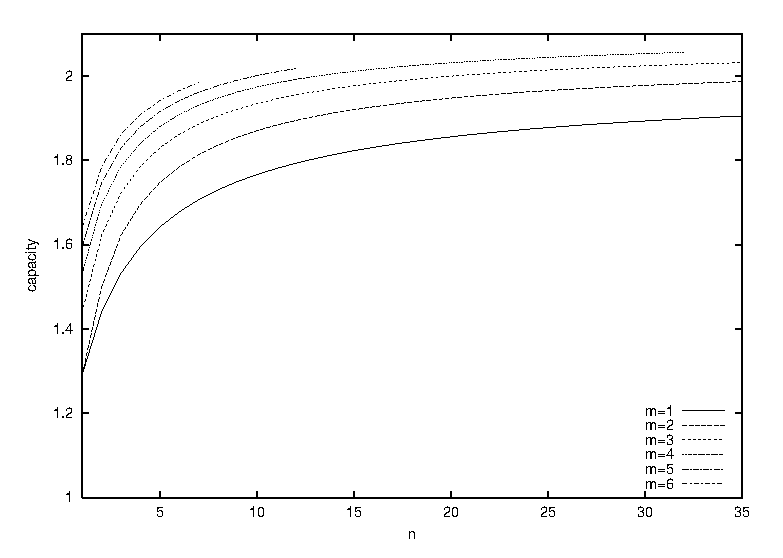
\includegraphics[height=6.8cm]{capsmall.eps}
  \label{fig:cap}
\end{figure*}

To give an impression of the amount of (machine) resources required
for the calculations: The run of the admissible shape algorithm for
$m=6$ and $n=7$ needed about three gigabytes of memory. The grid
$P_{6,7}$ has $370252552$ admissible shapes. We generated them in
lexicographical order with respect to the pairs of starting heights
and volumes. This way, never more than $15\%$ of the admissible shapes
had to be kept in memory simultaneously.  Notice that more than 400
megabytes (of the 3 gigabytes in total) where needed just to store the
\emph{numbers} of triangulations of the admissible shapes in the
memory. The CPU time used for the computation was about 25 hours.  Our
computations were performed on a SUN UltraAX MP machine equipped with
four 448 MHz UltraSPARC-II processors (of which we used only one) and
4 gigabytes main memory.

For very small parameters, Meyer~\cite{Meyer} has enumerated all
unimodular triangulations by Avis and Fukuda's reverse search method
(sketched at the beginning of this section) and checked them for
regularity. Table~\ref{tab:regsmall} shows the results. While for
these small parameters irregular triangulations are quite rare, the
picture changes drastically when~$m$ and~$n$ get larger, see
Section~\ref{sec:trias}. 

\begin{table}[ht]
  \centering
  \begin{tabular}{crrr}
    \hline
    $m\times n$ &
    \multicolumn{1}{c}{$\#$ triangulations} &
    \multicolumn{1}{c}{$\#$ irregular} &
    \multicolumn{1}{c}{fraction} \\
    \hline
    $3\times 3$ & 46456     & 4       & .000086 \\
    $3\times 4$ & 2822648   & 502     & .000178 \\
    $3\times 5$ & 182881520 & 63528   & .000347 \\
    $4\times 4$ & 736983568 & 1553020 & .002107 \\
    \hline
  \end{tabular}
  \caption{Number of regular triangulations of small grids.}
  \label{tab:regsmall}
\end{table}



%%% Local Variables:
%%% mode: latex
%%% TeX-master: "bcc_ct"
%%% End:


